\documentclass[12pt,letterpaper,twoside]{amsart}
\usepackage[latin1]{inputenc}
\usepackage{amsmath}
\usepackage{amsfonts}
\usepackage{graphicx}
\usepackage{amssymb}
\usepackage{multicol}
\usepackage{ulem}
\newcounter{example}
\newcounter{exercise}
\newcounter{problem}
\newcommand{\example}{\bigskip \noindent {\large {\sc Example \arabic{example}:}} \addtocounter{example}{1}}
\newcommand{\exercise}{\bigskip \noindent {\large {\sc Exercise \arabic{exercise}:}} \addtocounter{exercise}{1}}
\newcommand{\problem}{\bigskip \noindent {\large {\sc Problem \arabic{problem}:}} \addtocounter{problem}{1}}
\newcommand{\tech}{\marginpar{\vskip 10mm \begin{center}\includegraphics[width=0.25in]{calculatorimagesmall.eps} \end{center}}}
\newcommand{\solution}{\medskip \noindent {\bf Solution: }}
\newcommand{\R}{\mathbb{R}}





\begin{document}

\sffamily

%%%%  switch the commenting on this line and the next \chapter{Introduction}
\begin{center} {\LARGE Spring-Mass Systems} \end{center}

\setcounter{example}{1}
\setcounter{exercise}{1}

In this chapter we study in depth a classic application of second-order constant coefficient systems.  We will model the behaviour of a mass attached to a freely-moving end of an ideal spring, possibly subject to a damping effect (imagine the spring and mass are submerged in molasses).

We will usually not show all the steps involved in solving each initial value problem in this chapter.  The reader is strongly encouraged to keep a pencil and paper handy in order to fill in all the missing steps.

Let us begin with a figure representing our physical system:

\begin{center}
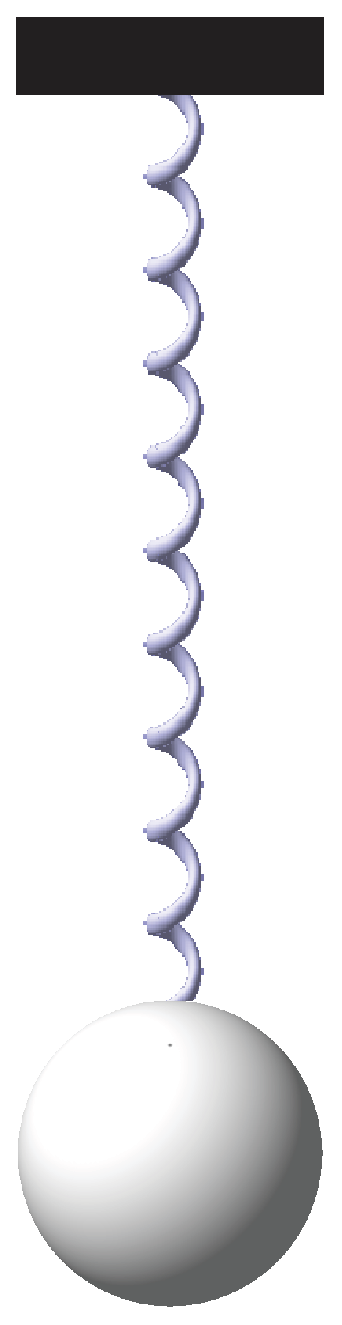
\includegraphics[width=3in]{springmass1.eps}
\end{center}

The free end of the spring is allowed to move, and we need to impose coordinates on the figure to measure this motion.  There are many ways we could choose to do this.  The natural point to choose as an origin is the {\bf rest position} of the free end of the spring -- that is to say, the point where the free end sits when the spring is not in a state of internal tension.  From this point, we can measure the displacement of the free end of the spring, and we shall adopt the convention that a stretched spring corresponds to a positive displacement, while a compressed spring corresponds to a negative displacement.

\begin{center}
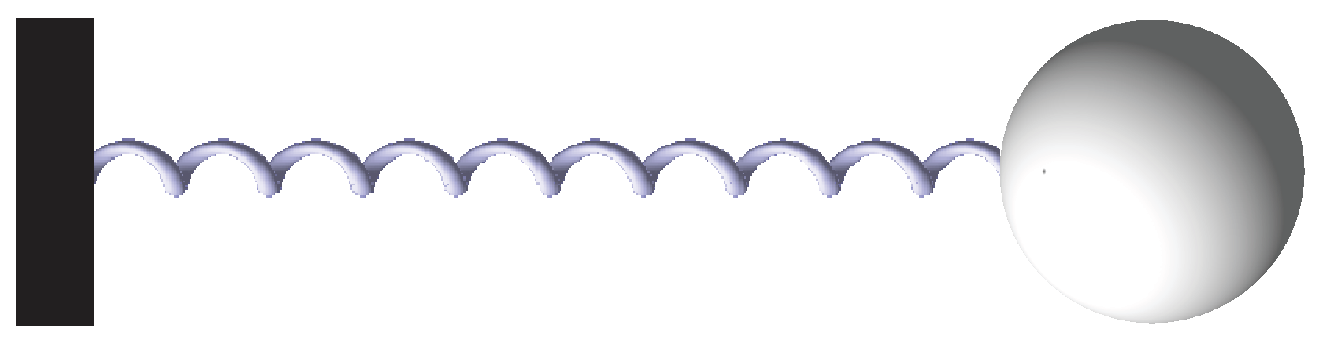
\includegraphics[width=3in]{springmass2.eps}
\end{center}

To model the physical behaviour of this system, our starting point is Newton's second law, $F=ma$ (force equals mass times acceleration).  If we let $y(t)$ denote the displacement of the free end of the spring from it's rest position as a function of time, then the acceleration is given by $\ddot{y}$.  There will also be at least two forces acting on the mass: the spring's restoring force, which Hooke's Law tells us we can model by assuming it is proportional to the displacement from rest position: $F_s = -ky$.  (Here, the spring constant $k$ is positive, and the direction of the spring's restoring force is in the direction opposite the displacement.  Also, we will model the damping force by assuming it is proportional to the velocity of the mass, and in the opposite direction: $F_d = -C\dot{y}$.  Let us denote any other external driving force by $F_e$.  Suppose this driving force is described by a function of time, $F_e=f(t)$.  With these conventions we have:
\[ ma=F_s+F_d+F_e\]
or
\[ m \ddot{y} = -ky - C \dot{y}+f(t),\]
which we rearrange as
\[ m \ddot{y} + C \dot{y} + k y = f(t).\]
We now see that this is a second order constant coefficient linear ODE, so we can study the behaviour of this system using the mathematical techniques now available to us.  

A standard choice of units for force would be Newtons, and a standard choice for measuring displacement $y$ would be meters.  Thus the spring constant could have units of $\frac{N}{m}$, indicating that the magnitude of the spring's restoring force is $k$ Newtons for each meter the spring is displaced from rest position.  If these units are used, then the last term on the left side of our ODE will have units of Newtons, which is consistent with the kind of units we would see on the right side of the equation for an external driving force $F_e$.  To maintain consistency with the other terms on the left side of the equation, we should select mass $m$ to be measured in kilograms, and time should be measured in seconds; that way the units of $m\ddot{y}$ will be $\frac{kg \cdot m}{s^2}$, which are the same as Newtons.  Similarly, the units of the damping coefficient will have to be $\frac{N \cdot s}{m}$.

\example Consider a mass of $3 \ kg$ attached to the end of a spring with spring constant $15 \frac{N}{m}$.  If there is no damping or outside driving force, and the mass is initially stretch $0.05 \ m$ from its rest position then released, determine how long it will take before the spring first returns to its rest position.  What will the velocity be at that instant?

With the parameters $m=3$, $C=0$ and $k=15$, and the driving force $f(t)=0$, we are faced with the differential equation
\[ 3 \ddot{y} + 15 y = 0,\]
and the initial conditions $y(0)=0.05$ and $y'(0)=0$.  The solution of this IVP is
\[ y(t) = 0.5 \cos (3t).\]
The free end of the spring will be at the rest position when $y(t)=0$, which will occurs when $3t = \frac{\pi}{2}+n\pi$, or $t=\frac{(2n+1)\pi}{6}$.  The smallest positive solution will be $t=\frac{\pi}{6}\approx 0.524 \ s$.  At that instant, the velocity will be $y'\left( \frac{\pi}{6} \right) = 1.5 \sin \left(\frac{\pi}{2} \right) = 1.5 \frac{m}{s}$.
\qed

\exercise A mass $m$ is attached to the free end of a spring with spring constant $k$, and the system is subject to a damping coefficient $C$.  The spring is stretched $0.05$ meters from it's natural length and released.  Determine how long it will take for the mass to return it it's natural length for each of the following sets of conditions.

{\bf (a)} $m=3, \ C=6, \ k=30$

{\bf (b)} $m = 3, \ C=9, \ k=6$

{\bf (c)} $m=3, \ C=6 , \ k=3 $

\bigskip
The following graphs illustrate the various solutions $y(t)$ from the previous example and the previous exercise.

\begin{center}
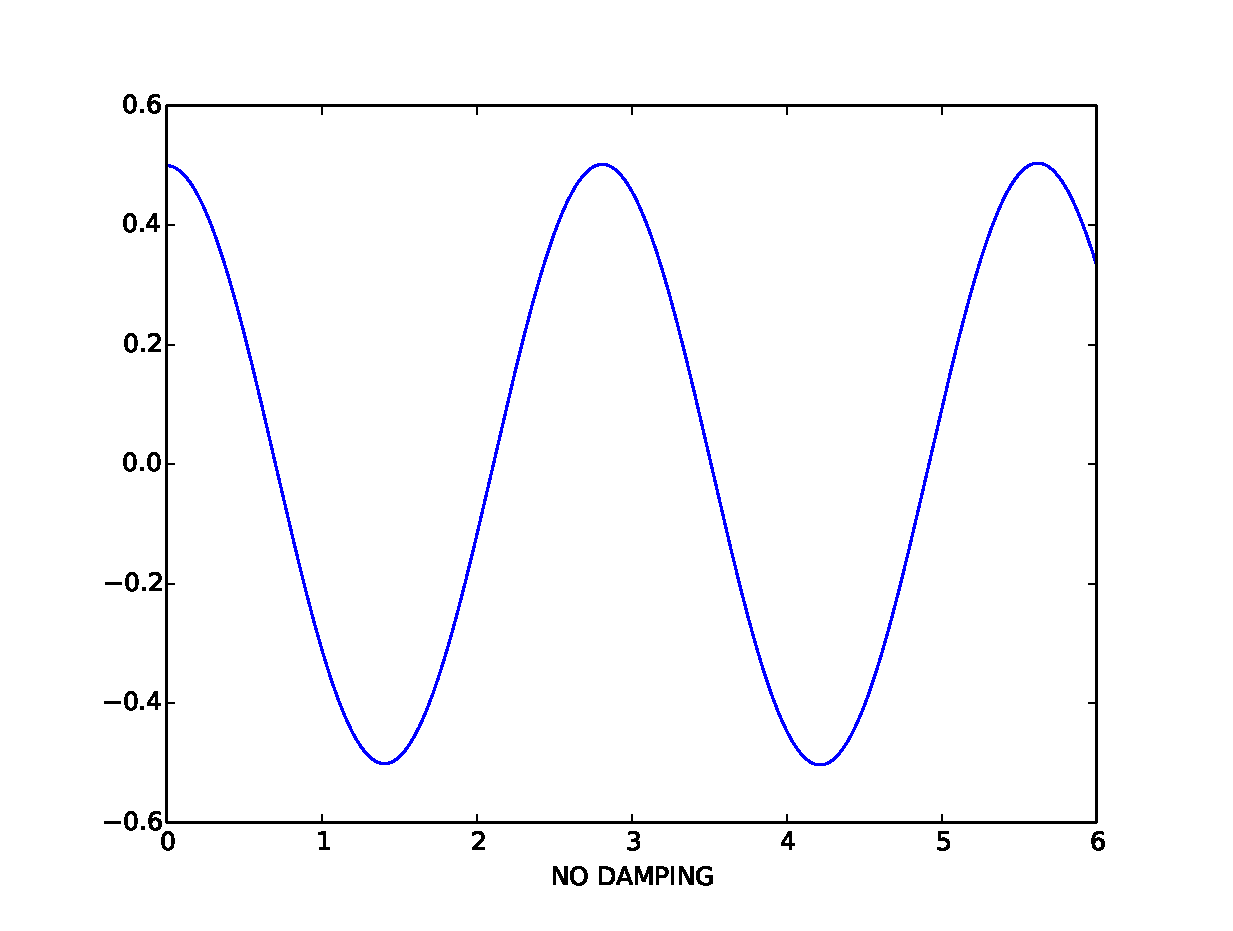
\includegraphics[width=2in]{nodamping.eps}
\hspace{0.25in}
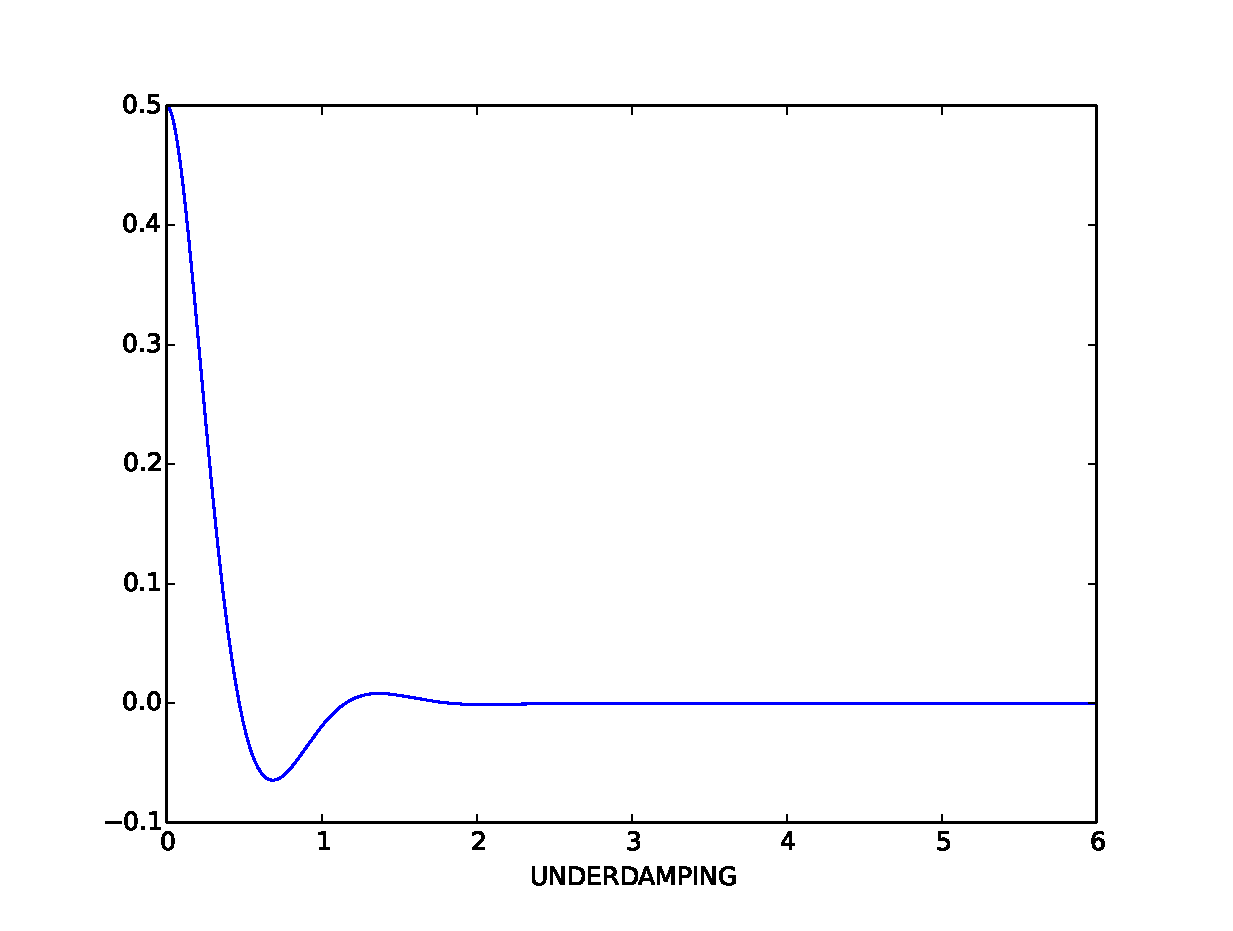
\includegraphics[width=2in]{underdamping.eps}

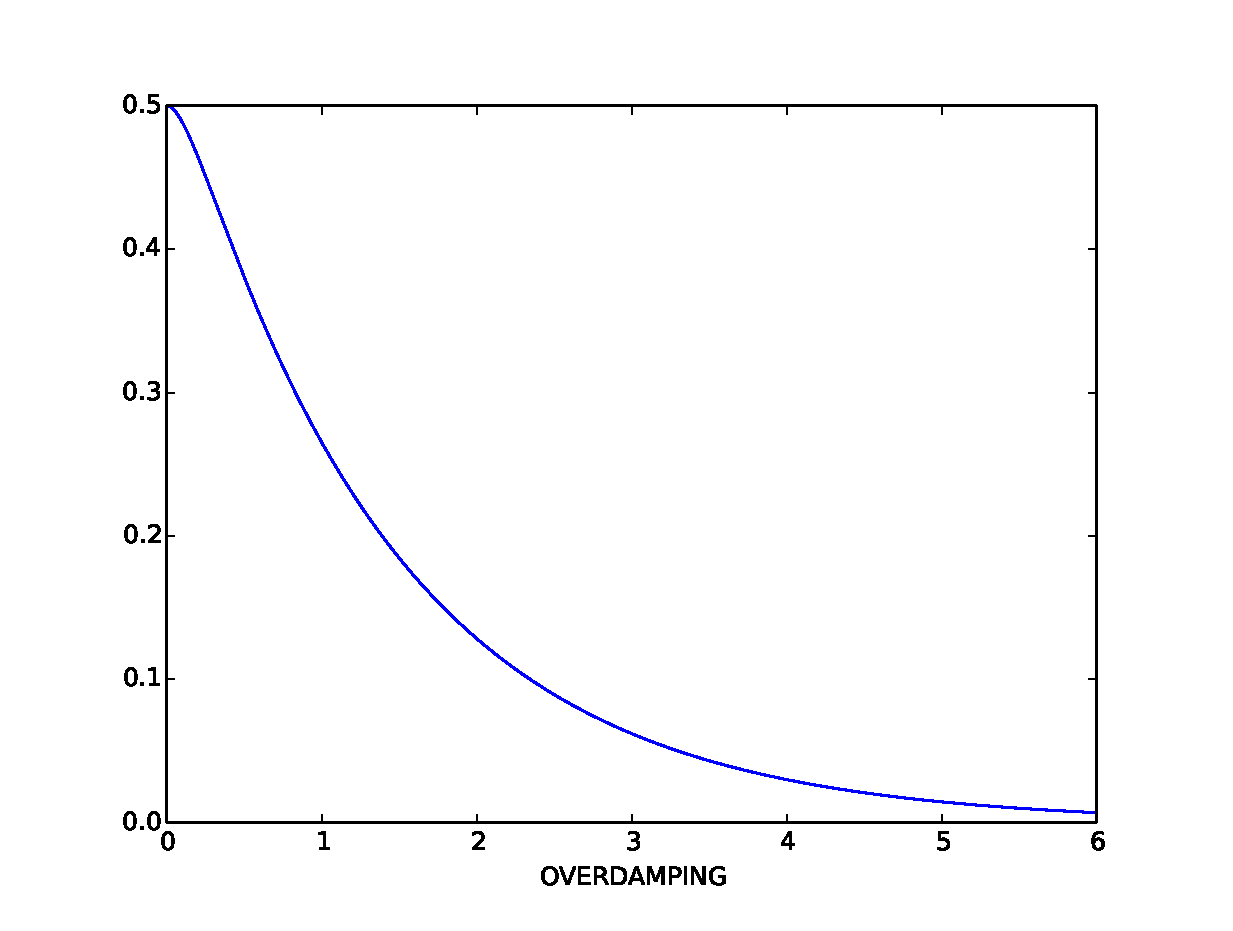
\includegraphics[width=2in]{overdamping.eps}
\hspace{0.25in}
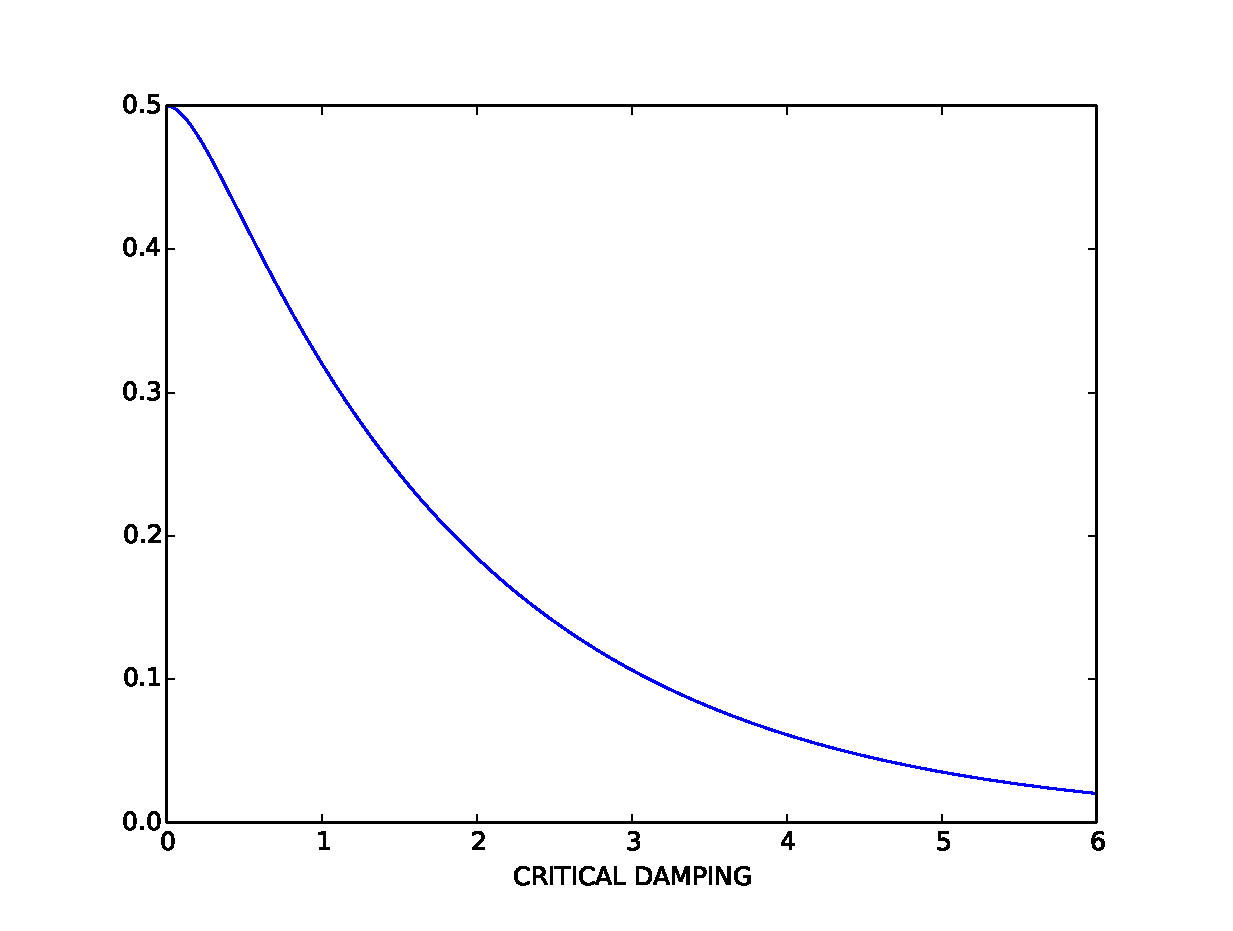
\includegraphics[width=2in]{criticaldamping.eps}
\end{center}

The captions for these graphs also include terminology which we will explain now.  The term in the first graph, {\bf no damping}, should be self explanatory.  Notice that the mass oscillates infinitely many times, always returning to the same maximum displacement as on the previous cycle.

The term describing the second graph, {\bf underdamping}, indicates that even though the magnitude of the oscillations decreases, the damping coefficient is too small (relative to the other parameters) to stop the solution from oscillating forever -- regardless of the initial conditions.  That is to say, no matter how small the initial displacement, or whether there is any initial velocity imparted, the solution will always oscillate through the rest position infinitely many times.  This is because the general solution has the form $y=A e^{-t} \cot(3t)+B e^{-t} \sin(3t)$, and any initial condition (other than the trivial one $y(0)=\dot{y}(0)=0$) will result in infinitely many such oscillations.

This stands in stark contrast to the third situation, which is described as {\bf overdamping}.  In this setting, the damping coefficient is so large that {\it no initial displacement} can cause more than one oscillation!  We can see this by analyzing the form of the general solution: $y(t) = A e^{-t}+Be^{-2t}$.  If we factor out $e^{-2t}$, we can write this as $y(t)=e^{-2t}(Ae^t+B)$, which will only be zero when $t=\ln \left(\frac{-B}{A} \right)$.  Depending on the choice of initial conditions, this value of $t$ may or may not exist, and even if it does exist, it may not be positive, in which case it would not be relevant to our model of the situation.

The last graph looks very similar to the naked eye, but we have given it a different name: {\bf critical damping}.  That is because this is the borderline case -- if the damping coefficient is reduced by any small amount whatsoever, the situation will switch to underdamping.  Also, the form of the general solution is slightly different, as the double root of the characteristic equation produces $y(t)=Ae^{-t}+Bte^{-t}$.  For this kind of function, the equation $y(t)=0$ definitely has a solution -- when $t=\frac{-A}{B}$ -- though this may still be a negative value and thus irrelevant to the model.

These differences in behaviour depend on the general solution of the equation $m\ddot{y}+C \dot{y} + ky =0$, which in turn is determined by the characteristic equation.  We can therefore use the characteristic equation to classify the type of damping in any setup.  To obtain infinitely many oscillations, our general solution must contain sinusoidal functions, and those occur when the characteristic equation has complex roots with non-zero imaginary parts; there will be no sinusoidal behaviour if the roots are real.  The borderline situation of critical damping is precisely the case of a double root.  If we solve the characteristics equation using the quadratic formula, 
\[ r = \frac{-C \pm \sqrt{C^2-4mk}}{2m},\]
then we can detect the types of solutions by looking directly at the discriminant (the expression inside the square root), as there will be real roots when the discriminant is positive (or zero) and complex roots when the discriminant is negative.  A zero discriminant is the borderline case.

\begin{center}
\fbox{
\begin{minipage}{3in}
A spring-mass system modelled by the ODE
\[ m\ddot{y}+C\dot{y}+ky=f(t)\]
exhibits:

{\bf No damping} if $b=0$;

{\bf Underdamping} if $C^2-4mk<0$;

{\bf Critical Damping} if $C^2-4mk=0$;

{\bf Overdamping} if $C^2-4mk>0$.

\end{minipage}
}
\end{center}

\exercise Classify the type of damping for each of the following situations.
\begin{enumerate}
\item $m=2, \ C=12, \ k=16$
\item $m=2, \ C=12, \ k=18$
\item $m=3, \ C=12, \ k=18$
\item $m=2, \ C=8, \ k=16$
\end{enumerate}

\exercise Suppose a mass of $4 \ kg$ is attached to the free end of a spring whose spring constant is $k=10 \frac{N}{m}$.  Find the exact value of the damping coefficient $C$ that will result in criticial damping.


Next we turn our attention to what happens when we introduce an external driving force.

\example A mass of $2 \ kg$ is hung from a spring whose spring constant is $34 \frac{N}{m}$.  The other end of the spring is anchored to the ceiling.  The system is subject to damping given by the constant $C=4\frac{N\cdot s}{m}$.  Gravity acts on the mass and, if not for the spring holding it, would accelerate the mass at $9.8 \frac{m}{s^2}$.  The mass is pushed up so that the spring is compressed o.1 meters from its natural length.  Then the mass is released.  Determine the long-term behaviour of the mass (i.e. $\lim_{t \rightarrow \infty} y(t)$).

The external driving force due to gravity acts downward on the mass, so it's effect is to lengthen the spring.  The magnitude of this force is $F_e = mg = (2 \ kg) \left(9.8 \frac{m}{s^2} \right) = 19.6 \ N$.  Our initial value problem is thus:
\[ 2 \ddot{y} + 4 \dot{y} +17 y = 19.6, \ \ \ y(0)=-0.3, \ \ \ \dot{y}(0)=0.\]
(Note that since we are treating the downward force of gravity as being in the positive direction, the initial displacement of the compressed spring must therefore be negative.)

The solution of this IVP is
\[ y(t)= \frac{9.8}{17} + \frac{81}{17}e^{-t} \cos(4t) + \frac{81}{680}e^{-t} \sin(4t).\]
From this, we see that
\[ \lim_{t \rightarrow \infty} y(t) = \frac{9.8}{17}.\]
That is to say, in the long term the mass settles toward a position that is $\frac{9.8}{17}\approx 0.58 \ m$ below the spring's natural rest position.
\qed

The position that the the mass (i.e. the free end of the spring) tends toward in the previous example is called the {\bf equilibrium position} because that is the position where the forces due to gravity and spring are in equilibrium with one another -- the downward force due to gravity is equal in magnitude to the upward force of the spring.  The reader should verify that the constant function $y(t)=\frac{9.8}{17}$ is an equilibrium solution of the differential equation in that example.

\example The spring-mass system in the previous example begins at rest in the equilibrium position, where spring and gravitational forces are balanced.  An earthquake then begins to shake the building up and down, imparting a force on the system that is transferred to the mass.  If this force is modelled by the function $f(t)=0.2 \sin(0.04t) \ N$, find formula for $y(t)$, and graph the solution over the time interval $0 \leq t \leq 300$.

We need to solve the IVP:
\[ 2 \ddot{y} + 4\dot{y} + 34 y = 19.6 + 0.02 \sin(0.04 t), \ \ \ y(0)=\frac{9.8}{17}, \ \ \ \dot{y}(0)=0.\]

The solution is given by the formula
\[ y(t) = \frac{9.8}{17}+A \cos(0.04t)+B\sin(0.04t)+Ce^{-t}\cos(4t)+De^{-t}\sin(4t),\]
where $A \approx -2.77 \cdot 10^{-6}$, $B \approx 5.88\cdot 10^{-4}$, $C\approx 2.77 \cdot 10^{-6}$ and  $D \approx -5.19 \cdot 10^{-6}$.  This a a graph of the functions with these rounded coefficients:

\begin{center}
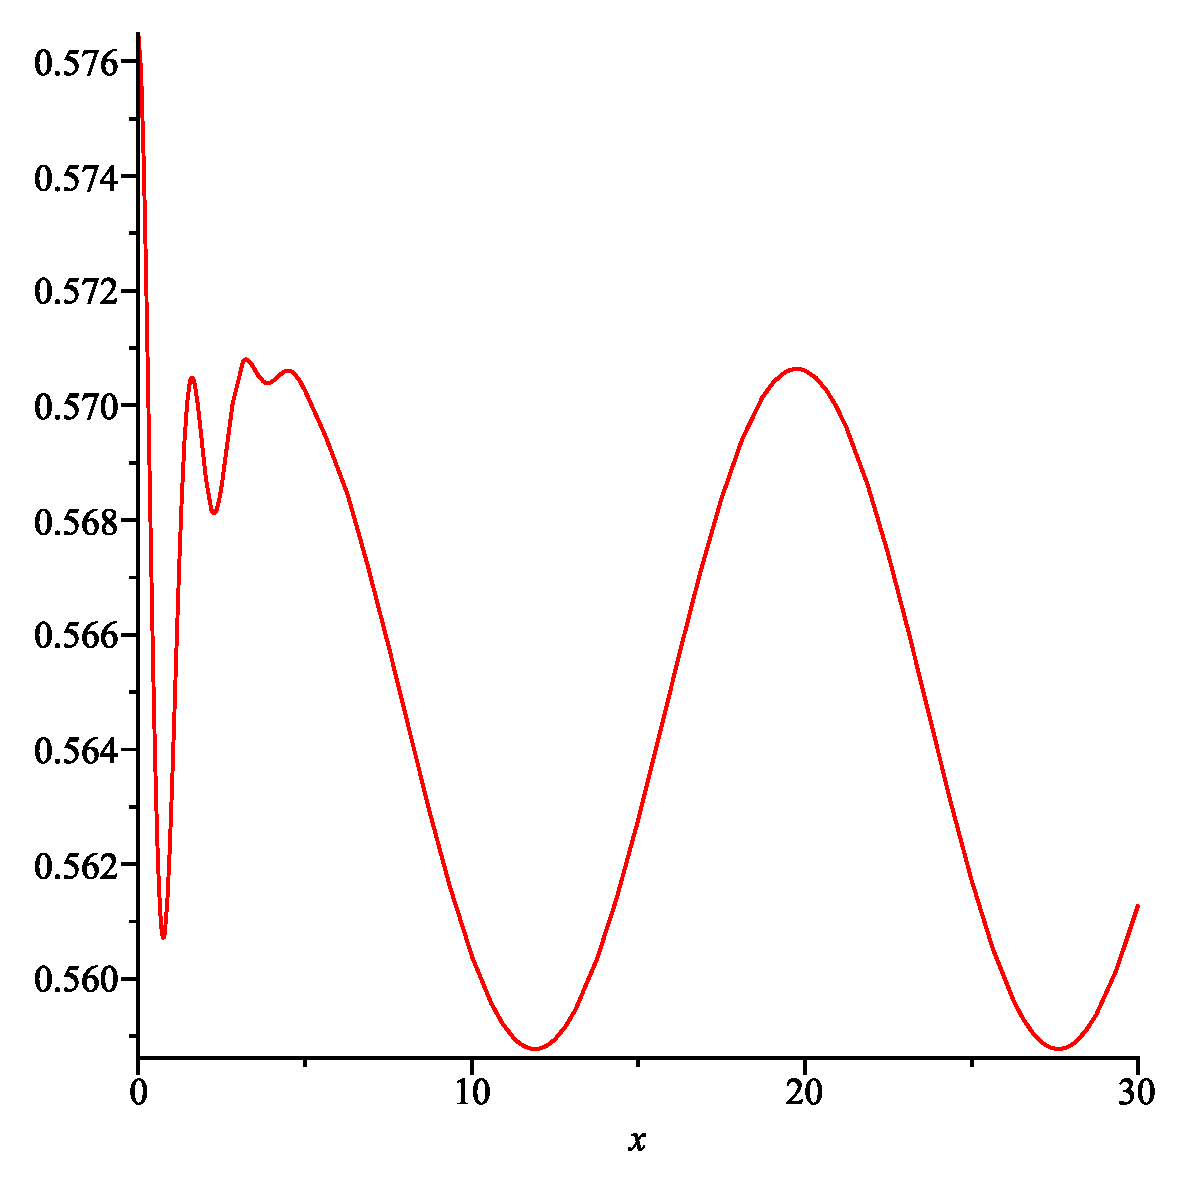
\includegraphics[width=2in]{sinusoidaldriving.eps}
\end{center}

Notice that in each of the examples we've explored so far in this chapter, we have encountered solutions of the form
\[ y(t) = y_S(t) + y_T(t),\]
where $y_S$ is periodic and $y_T(t) \rightarrow 0$ as $t \rightarrow \infty$.  Thus the long-term behaviour of $y$ matches whatever the long-term behaviour is of $y_S$, while $y_T$ becomes negligible.  For this reason, the term $y_T$ is called a {\bf transient solution} of the IVP, while $y_S$ is called the {\bf steady-state solution}.  For example, the solution of the IVP
\[ \ddot{y} + 2 \dot{y} + y = \cos(t), \ \ \ y(0)=0, \ \ \ y'(0)=0\]
is the function $y(t)=\frac{1}{2}\sin(t)-\frac{1}{2}te^{-t}.$
The transient solution is $y_T=-\frac{1}{2}te^{-t}$, and the steady-state solution is $y_S=\frac{1}{2}\sin(t)$.  The following graph of $y$ and $y_S$ indicates the increasing similarity between these function as $t$ increases.

\begin{center}
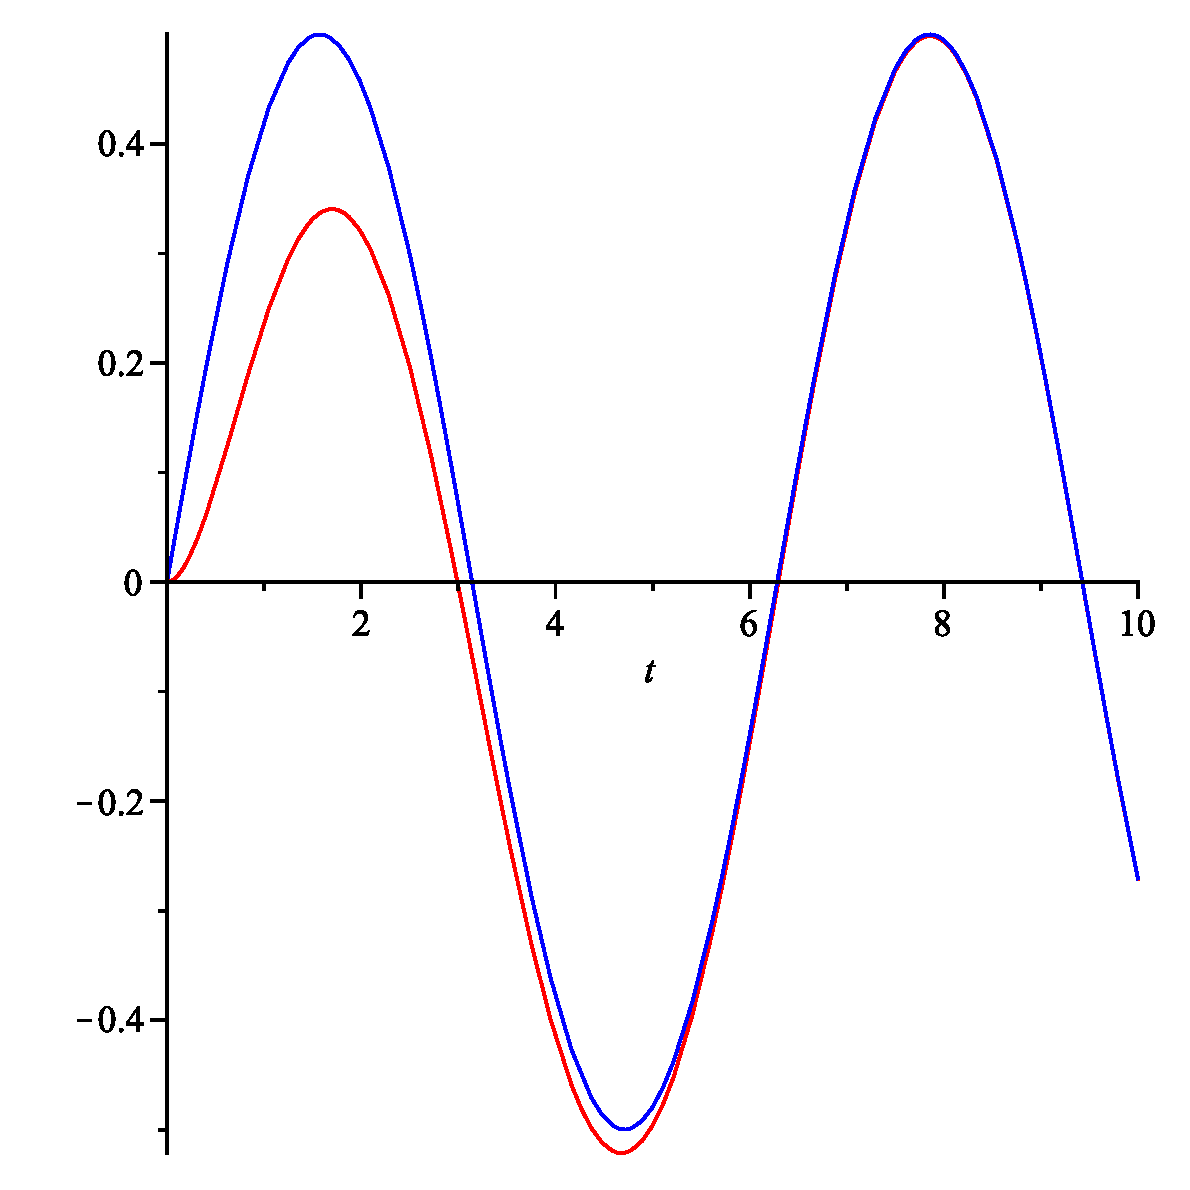
\includegraphics[width=2in]{steadystatecomparison.eps}
\end{center}

We have one last topic to explore in this chapter which will arise in the following example.

\example Suppose a spring-mass system is modelled by the IVP
\[ \ddot{y} + y = \sin(\omega t), \ y(0)=0, y'(0)=0.\]
Explore the consequences of various values of the driving frequency $\omega>0$ on the solutions of this IVP.

The characteristic equation is $r^2+1=0$, which has roots $r=\pm i$.  Therefore the solution of the related homogeneous equation is 
\[ y_h (t) = A \cos(t) + B \sin(t).\]
We will need to be careful when we guess the form of a particular solution to non-homogeneous equation, because the form of our guess depends upon the value of $\omega$.

First, if $\omega \neq 1$, then we guess $y_p(t)=C \sin(\omega t) + D \cos(\omega t)$, and the method of undetermined coefficients leads us to the solution
\[ y_p(t) = \frac{1}{1-\omega^2} \sin\left( \omega t \right). \]
Therefore the general solution of the non-homogeneous problem is
\[ y(t) = \frac{1}{1-\omega^2} \sin \left( \omega t \right) + A \sin(t) + B \cos(t),\]
and the initial conditions $y(0)=\dot{y}(0)=0$ imply $A=\frac{\omega}{1-\omega^2}$ and $B=\frac{1}{\omega^2-1}$.  Consequently we have
\[ y(t) = \frac{1}{1-\omega^2} \sin \left( \omega t \right) + \frac{\omega}{1-\omega^2} \sin(t) + \frac{1}{1-\omega^2} \cos(t).\]


Notice that the amplitude coefficients here all become larger as $\omega$ gets closer to $1$.

On the other hand, if we start out with $\omega = 1$, then the initial guess for a particular solution of the non-homogeneous equation will have the form $y_p(t) = C t \cos(t) + D t \sin(t)$, and the reader shoudl verify that this eventually leads to the complete solution
\[ y(t) = -\frac{1}{2} t \cos (t) + \frac{1}{2} \sin(t).\]
In this case, as time progresses, the magnitude of the oscillations increases without bound.
\qed

The phenomenon explored in the last example is called {\bf resonance}.  The idea is that the spring-mass system has a natural frequency at which it wants to oscillate.  If the driving force oscillates at close to this frequency, the resulting oscillations in the system will be larger in amplitude than they would be if the frequencies were not close (even if the amplitude of the driving force is not changed).  If the driving force is applied at exactly the resonant frequency, then the oscillations will grow in magnitude instead of tending to a steady-state (i.e. periodic) behaviour.



%% Cut below here for the book form.

\newpage
\begin{center} {\LARGE Problems} \end{center}

\setcounter{problem}{1}

\problem Prove that, if there is no external driving force and any damping at all (i.e. $C>0$) for a spring-mass system, then $\lim_{t \rightarrow \infty} y(t)=0$.

\problem Consider a critically damped spring-mass system subject to the following parameters: $m=2, \ C=8, \ k=8$.  If the initial displacement is $y(0)=1$ and the initial velocity is $\dot{y}=v_0$, find a condition on $v_0$ that determines whether or not the spring will ever pass through its natural length during the time interval $t>0$.

\problem Repeat the previous problem for the overdamped spring-mass system: $m=2, \ C=10, \ k=8$.

\problem Consider a damped spring-mass system described by the IVP $\ddot{y}+2\dot{y} + 2y =\sin (\omega t)$, $y(0)=\dot{y}(0)=0$.  Explore the consequences of various frequencies $\omega >0$ for the external driving force.  What effect will there be on the amplitudes of the steady-state solutions?

 






\end{document}